%!TEX root = ../main.tex

\section{Problema 5: Integración Numérica}
Se tiene la integral
\[
I = \int_0^1 \frac{4}{1 + x^2} dx = \pi.
\]

\begin{itemize}
    \item Use las reglas compuestas del punto medio, del trapecio y de Simpson para aproximar $I$ para varios tamaños de paso de integración $h_n = 1/n$, $n = 10, 50, 100, 250, 500, 1000, 1500, 2000$. Grafique el logaritmo del error absoluto versus $n$ para cada paso. Describa el efecto de redondeo de los errores cuando $h \to 0$.
    \begin{solution}
        Al implementar los distintos métodos de integración numérica, obtuvimos la siguiente gráfica para los diferentes tamaños de paso:

        \begin{figure}[H]
         \centering
         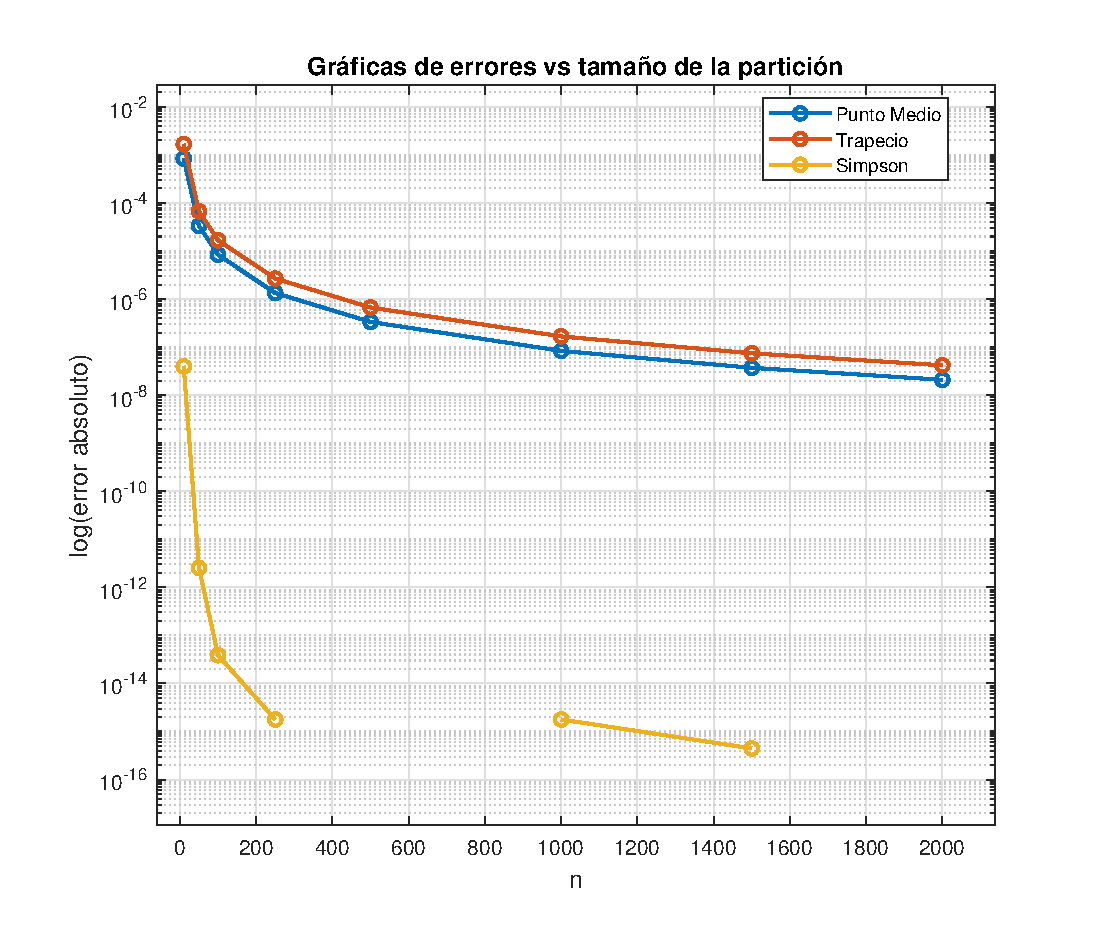
\includegraphics[scale=0.7]{Graficas/Punto_5_a.eps}
         \end{figure}  

         Podemos observar que para las reglas del punto medio y del trapecio el comportamiento del logaritmo del error absoluto versus n, el error decae de manera exponencial, Para el caso de la regla de Simpson obtenemos valores que no parecen seguir una tendencia clara, pues para, por ejemplo una partición de 500 puntos o 2000 puntos, se tiene un error tan pequeño que la maquina lo reporta como 0.

         Ahora, si aumentamos el tamaño de las particiones, vemos que el error empieza a aumentar en el caso de la regla de Simpson, lo cual puede deberse a que éste metodo requiere de más operaciones, y a medida que aumenta el número de puntos se va propagando el error. Para el caso de las reglas del trapecio y del punto medio, se puede observar que el redondeo del error es más estable. Esto se puede observar en la siguiente gráfica, en la que comparamos el logaritmo del error absoluto contra el logaritmo del tamaño de la partición

        \begin{figure}[H]
        \centering
        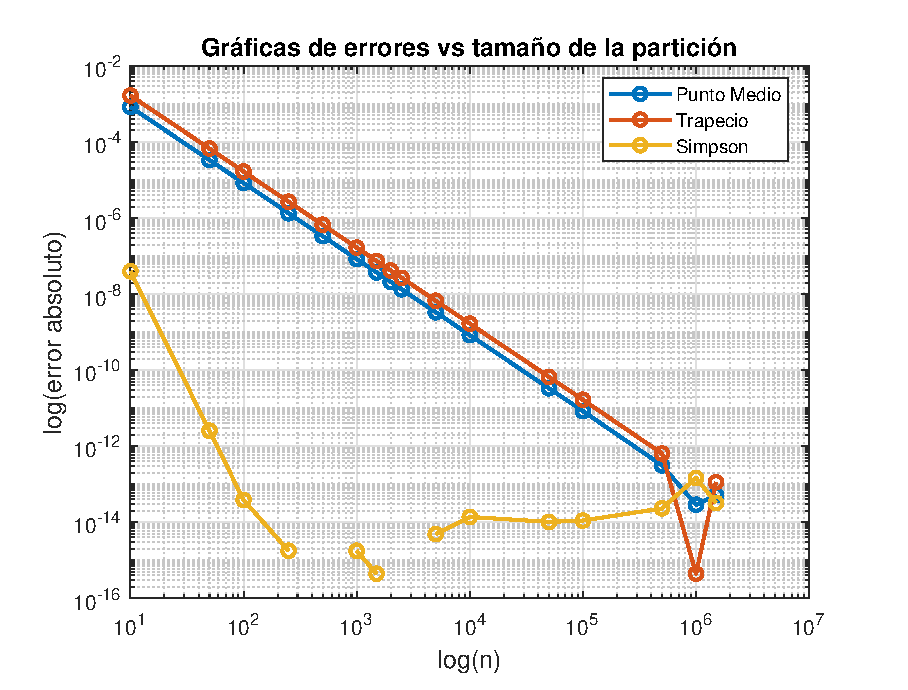
\includegraphics[scale=0.8]{Graficas/Punto_5_a2.eps}
        \end{figure}  

    \end{solution}
    \item Implemente el método de integración de Romberg para calcular $I$. Grafique el logaritmo del error en los términos diagonales en la tabla de extrapolación versus $\log h$. Verifique sus resultados con la teoría.

    \begin{solution}
        Al implementar el método de Romberg, la gráfica de los errores versus log(h), es la siguiente: 

        \begin{figure}[H]
        \centering
        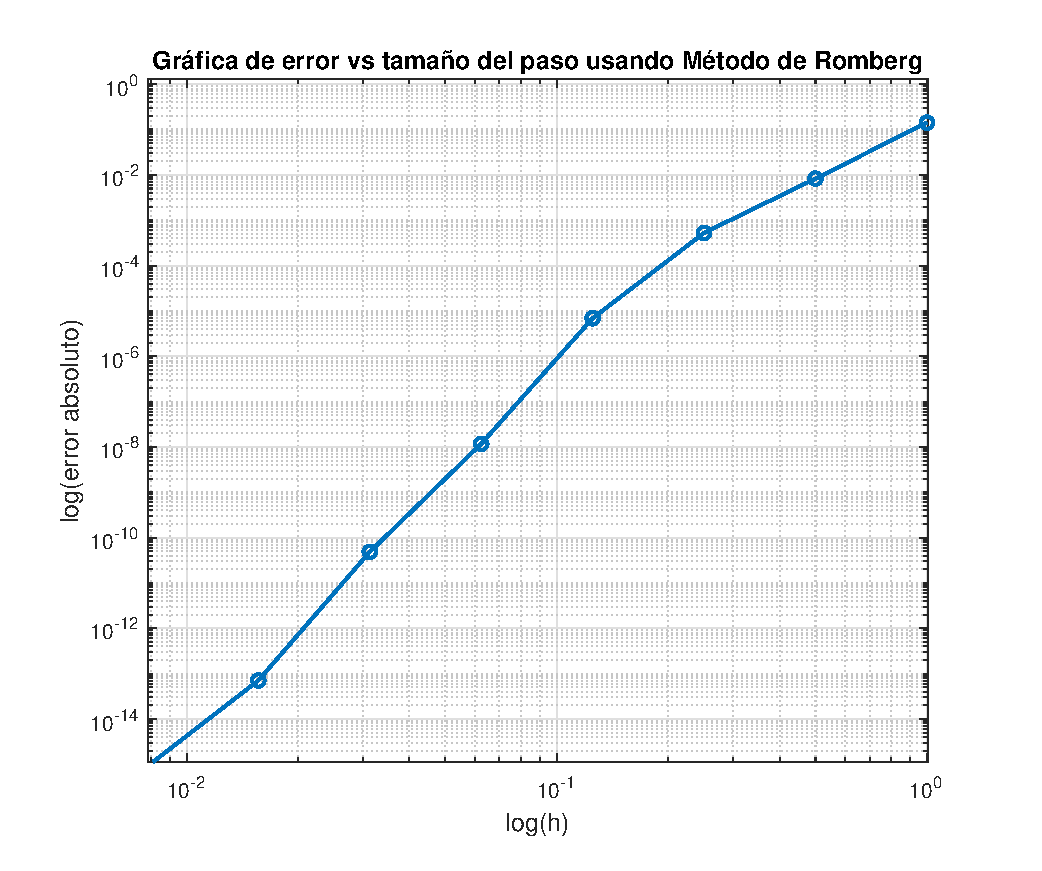
\includegraphics[scale=0.65]{Graficas/Punto_5_b.eps}
        \end{figure}  

        Según la teoría, el error de cada aproximación es del orden de $O(h_K^{2K})$, donde $K$ es la fila correspondiente a la aproximación en la tabla de extrapolación, en nuestro caso,  debemos obtener que el error es del orden de $O(1/2^k)$, con lo cual podriamos esperar que a medida que el tamaño del paso aumenta, el tamaño del exponente en la gráfica obtenida, se duplique. Notamos que éste comportamiento se pude apreciar de manera aproximada en la gráfica, por lo cual es consistente con la teoría.
    \end{solution}    
\end{itemize}
